\documentclass[tikz]{standalone}
\usepackage{tikz}
\usepackage[AutoFakeBold=true,AutoFakeSlant=true]{xeCJK}
\usepackage[zihao=-4,UTF8,heading=true]{ctex}
\usepackage[simplified]{pgf-umlcd}
\usetikzlibrary{fit} %形状
\usetikzlibrary{positioning} %不加方向运算可能出错
\usetikzlibrary{arrows.meta} %箭头
\usetikzlibrary{calc}

\setCJKmainfont{微软雅黑}
\begin{document}
	\thispagestyle{empty}
    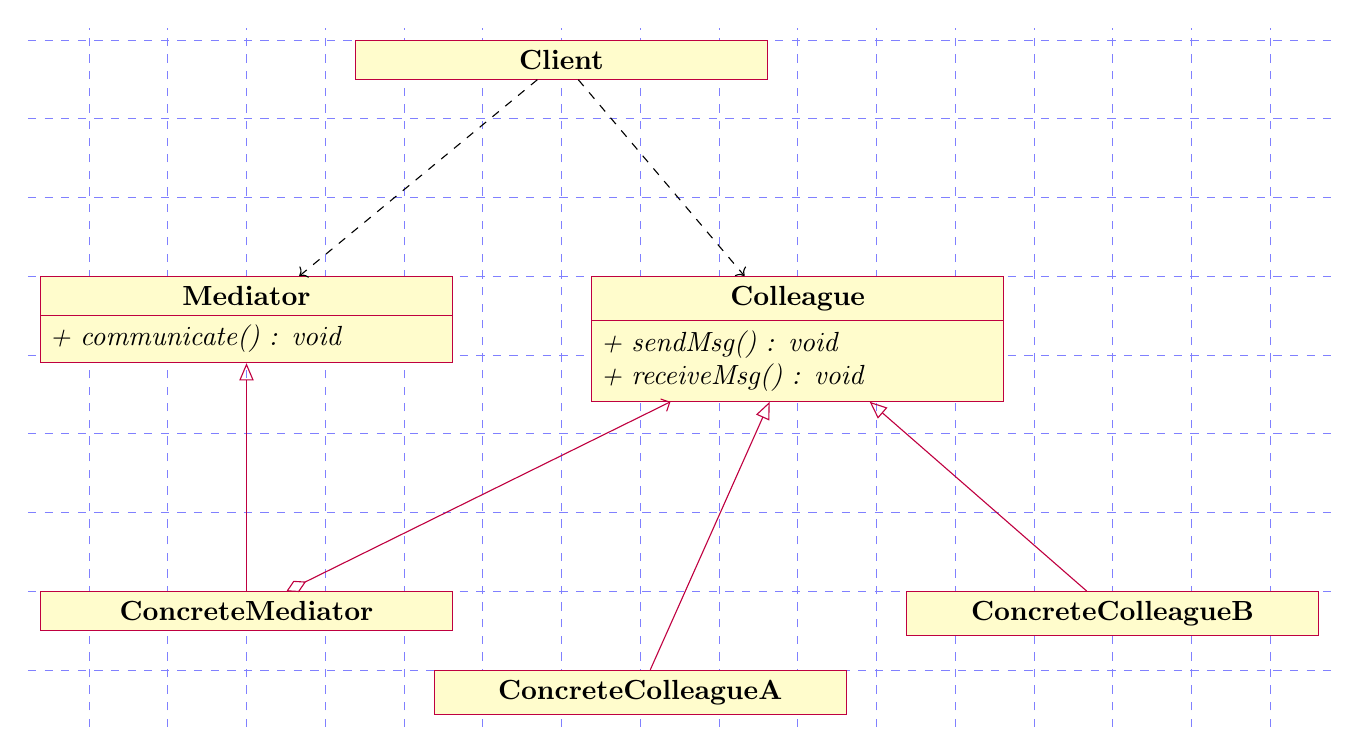
\begin{tikzpicture}[show background grid]
        \begin{class}[text width=5cm]{Mediator}{0,0}
            \operation[0]{+ communicate() : void}
        \end{class}
        \begin{class}[]{Colleague}{7, 0}
            \operation[0]{+ sendMsg() : void}
            \operation[0]{+ receiveMsg() : void}
        \end{class}
        
        \begin{class}[]{ConcreteMediator}{0, -4}
            \inherit{Mediator}
        \end{class}
        \begin{class}[]{ConcreteColleagueA}{5, -5}
            \inherit{Colleague}
        \end{class}
        \begin{class}[]{ConcreteColleagueB}{11, -4}
            \inherit{Colleague}
        \end{class}
        \aggregation{ConcreteMediator}{}{}{Colleague}
        \begin{class}[]{Client}{4, 3}
        \end{class}
        \draw [dashed, ->] (Client) -- (Mediator);
        \draw [dashed, ->] (Client) -- (Colleague);
    \end{tikzpicture}

\end{document}